\documentclass[14pt,a4paper]{extarticle}
\renewcommand{\rmdefault}{ftm}
\usepackage{amssymb,amsmath,amsthm,enumitem}
\usepackage{cmap}
\usepackage[utf8]{inputenc}
\usepackage[T1,T2A]{fontenc}
\usepackage[english,russian]{babel}
\usepackage{mathtext}
\usepackage{indentfirst}
\linespread{1.3}
\usepackage[left=3cm,right=1.5cm,top=2cm,bottom=2cm,bindingoffset=0cm]{geometry}
\usepackage{titlesec}
\usepackage{graphicx}
\usepackage{subfigure}
\usepackage{mathtools}
\usepackage{amssymb}
\usepackage{float}
\usepackage{sidecap}
\usepackage{wrapfig}
\usepackage{caption}
\usepackage{physics}
\usepackage{tensor}
\usepackage[hidelinks]{hyperref}
\usepackage{minted}

\addto\captionsrussian{\def\refname{СПИСОК ИСПОЛЬЗОВАННЫХ ИСТОЧНИКОВ}}



\makeatletter
\g@addto@macro\normalsize{%
	\setlength\abovedisplayskip{4.5ex}
	\setlength\belowdisplayskip{4.5ex}
	\setlength\abovedisplayshortskip{4.5ex}
	\setlength\belowdisplayshortskip{4.5ex}
}
\makeatother

\titleformat{\section}
{\normalfont\fontsize{14}{19}\selectfont}{\normalfont\hspace{1.25cm}\thesection}{1em}{}
\titleformat{\subsection}
{\normalfont\fontsize{14}{17}\selectfont}{\normalfont\hspace{1.25cm}\thesubsection}{1em}{}
\titleformat{\subsubsection}
{\normalfont\fontsize{14}{17}\selectfont}{\normalfont\hspace{1.25cm}\thesubsubsection}{1em}{}

\titlespacing*{\section}
{0pt}{4.5ex}{4.5ex}

\titlespacing*{\subsection}
{0pt}{4.5ex}{4.5ex}

\titlespacing*{\subsubsection}
{0pt}{4.5ex}{4.5ex}

\renewcommand{\bfseries}{\relax}

\makeatletter
\renewcommand\tableofcontents{%
	\normalfont\null\hfill\normalfont{\normalfont\contentsname}\hfill\null\par
	\@mkboth{\normalfont\contentsname}{\normalfont\contentsname}%
	\@starttoc{toc}%
}
\makeatother

\renewcommand{\labelenumi}{$\arabic{enumi})$}








\begin{document}
	\begin{titlepage}
	\begin{center}
		\large
		МИНИСТЕРСТВО ОБРАЗОВАНИЯ И НАУКИ\\ РОССИЙСКОЙ ФЕДЕРАЦИИ
		
		\vspace{0.5cm}
		
		МГТУ им Н.Э.Баумана
		\vspace{0.25cm}
		
		Факультет ФН
		
		Кафедра вычислительной математики и математической физики
		\vfill
		
		
		Соколов Арсений Андреевич\\
		\vfill
		
		
		{\LARGE Курсовая работа по дифференциальной геометрии\\[2mm]
		}
		\bigskip
		
		3 курс, группа ФН11-53Б\\
		Вариант 8
	\end{center}
	\vfill
	
	\newlength{\ML}
	\settowidth{\ML}{«\underline{\hspace{0.7cm}}» \underline{\hspace{2cm}}}
	\hfill\begin{minipage}{0.4\textwidth}
		Преподаватель\\
		\underline{\hspace{3cm}} Е.\,В.~Осипов\\
		«\underline{\hspace{0.7cm}}» \underline{\hspace{1.71cm}} 2019 г.
	\end{minipage}%
	\bigskip
	
	
	\vfill
	
	\begin{center}
		Москва, 2019 г.
	\end{center}
\end{titlepage}
\tableofcontents
\parindent=1.25cm
\clearpage


\section*{рпз}
\newpage
\section*{список исполнителей}
\newpage
\section*{реферат}
\newpage
\section*{введение}
\newpage

\section{Римановы пространства}
В механике и особенно в релятивистской физике тензоры широко применяют в $n$-мерных римановых пространствах, являющихся более общими, чем евклидовы \cite{Dimitrienko}. Дадим определение этих пространств, а затем покажем, как конструируются тензоры в них. Начнём с основополагающего понятия римановых пространств - элементарного многообразия.

\subsection{Элементарное многообразие}
Определение 1. Элементарным $n$-мерным многообразием называют такое множество $M^n$, каждой точке которого
взаимнооднозначно поставлен в соответствие упорядоченный набор чисел $(X_1...X_n)$ из некоторой связной области $\mathcal{D} \in \mathbb{R}^n$, т.е, задано биективное отображение $\varphi: M^n \longrightarrow \mathcal{D} \in \mathbb{R}^n$.

Координатами точки $\mathcal{M} \in M^n$ в системе координат $\mathcal{D}$ называют координаты $X^i \in \mathbb{R}^n$ ее образа $\varphi(\mathcal{M})$, изменяющиеся в области $\mathcal{D} \in \mathbb{R}^n$.
Если для множества $M^n$ имеется другое биективное отображение $\varphi': M^n \longrightarrow \mathcal{D} \in \mathbb{R}^n$, то координаты точки $\mathcal{M}$ в системах координат $\mathcal{D}$ и $\mathcal{D'}$, связаны соотношениями:

\begin{equation}\label{e1}
	X'^i = X'^i(X^j), \quad i,j=1\dots n,
\end{equation}

которые предполагают достаточное число раз дифференцируемыми и невырожденными, т.е. $\det (\pdv{X'^i}{X^j}) \neq 0, \forall X^i \in \mathcal{D}$.
Введём обозначения для якобиевых матриц преобразования, а также для их производных:

\begin{equation}\label{eq2}
	Q_{\; j}^{i} \equiv\left(\frac{\partial X'^{i}}{\partial X^{j}}\right), \quad P_{\; j}^{i} \equiv\left(\frac{\partial X^{i}}{\partial X'^{j}}\right), \quad P_{\; j k}^{i} \equiv \frac{\partial^{2} X^{i}}{\partial X'^{j} \partial X'^{k}},
\end{equation}

и кроме того будем использовать обозначения для частных производных:

\begin{equation}\label{eq3}
	\pdv{f}{X^i} \equiv f_{,i}, \quad \pdv{f}{X'^i} \equiv f_{|i} = P_{\; i}^j f_{,i}.
\end{equation}

Примером двумерного $(n = 2)$ элементарного многообразия $M^2$ являются поверхности в $\mathbb{R}^3$, на которых определены криволинейные координаты $X_1, X_2$ и которые заданы тремя функциями:

\begin{equation}\label{eq4}
	x^i = x^{i}(X^1, X^2), \quad i=1,2,3.
\end{equation}
\subsection{Касательное пространство}
Определение 2. Кривой $\mathcal{L}$ в многообразии $M^n$ называют отображение $\mathcal{L}: [\xi_1,\xi_2] \in \mathbb{R}^1 \longrightarrow M^n$, которое записывают в виде функции:
\begin{equation}\label{eq5}
	X^i = X^i(\xi) \quad \forall \xi \in [\xi_1, \xi_2], \quad X^i \in M^n.	
\end{equation}

Здесь $X^i$ - координаты точки $\mathcal{M} \in M^n, [\xi_1, \xi_2]$ - некоторый отрезок из $\mathbb{R}^1, (\xi_1 < \xi_2)$, а функции (\ref{eq5}) предполагаем непрерывно дифференцируемыми, по крайней мере, два раза.


Зафиксировав значение параметра $\xi \in [\xi_1,\xi_2]$, получим некоторую точку $\mathcal{M} \in \mathcal{L}$, в ней можно вычислить производные от функций (\ref{eq5}):
\begin{equation}\label{eq6}
	a^i = \dv{X^i}{\xi}.
\end{equation}

Определение 3. Упорядоченный набор $(a_1\dots a_n)$ производных (\ref{eq6}) называют компонентами касательного вектора $a^i$ в точке $\mathcal{M}$ кривой $\mathcal{L}$ в $ M^n $.

Если перейти к координатам $X'^i$ той же точки $\mathcal{M} \in \mathcal{L}$, то согласно (\ref{e1}) получаем, что компоненты касательного вектора $a'^i$ в этой системе координат будут иметь вид: $a'^i = \dv{X'^i}{\xi}$ и связаны с $a^i$ тензорным законом:
\begin{equation}\label{eq7}
	a'^i = Q_{\; j}^i a^j.
\end{equation}

Поскольку через фиксированную точку$\mathcal{M} \in M^n$ можно провести различные кривые $\mathcal{L}$, то, вообще говоря, в каждой точке $\mathcal{M}$ имеется множество упорядоченных наборов $(a_1\dots A_n)$. Определим операции с этими наборами.

Пусть имеется две кривые $\mathcal{L_\textup{1}}$ и $\mathcal{L_\textup{2}}$, заданные в виде функций $X_1^i(\xi), X_2^i(\xi)$, проходящие через точку $\mathcal{L}$, тогда можно построить два набора компонент касательных векторов $a_1^i = \dv{X_1^i}{\xi}$ и $a_2^i = \dv{X_2^i}{\xi}$.

Суммой компонент двух касательных векторов назовём набор
\begin{equation}\label{eq8}
	a_1^i + a_2^i = \dv{X_1^i + X_2^i}{\xi},
\end{equation}
который представляет собой компоненты касательного вектора к кривой $(X_1^i + X_2^i)(\xi)$ в данной точке $\mathcal{M}$.

Аналогично определяем произведение компонент $а^i$ на вещественное число $\lambda$:
\begin{equation}\label{eq9}
	\lambda a^i = \lambda \dv{X^i}{\xi} = \dv{\lambda X^i}{\xi}.
\end{equation}

Поскольку набор чисел $(a_1 ...a_n)$ является элементом пространства $\mathbb{R}$, то, выбрав базис $e_i$ в этом пространстве, можно построить сам касательный вектор $a$ в точке $\mathcal{M}$ кривой $\mathcal{L}: a = a^ie_i = a'^ie'_i$, где $e'_i = P_{\; i}^j e_j$ - новый базис.


Определение 4. Касательным пространством в данной точке $\mathcal{M}$ элементарного многообразия $M^n$ называют множество касательных векторов $а = a^ie_i$, построенных ко всевозможным кривым $\mathcal{L}$, проходящим через данную точку.


Теорема 1. Касательное пространство в любой точке $\mathcal{M} \in M^n$ является $n$-мерным линейным пространством, которое обозначают как $T_{\mathcal{M}}M^n$, а векторы $e$, образуют базис в нем.


\subsection{Определение риманова пространства}
Определение 5. Элементарное $n$-мерное многообразие $M^n$ называют римановым пространством $\mathbb{V}^n$, если в каждой точке $\mathcal{M} \in M^n$ с координатами $X^i$ задана матрица $g_{ij}$ $n$-го порядка, которая является

\begin{enumerate}
	\item симметричной,
	\item невырожденной: $\det (\tilde{g}_{ij}) \neq 0, \quad \forall X^i$,
	\item компоненты её являются непрерывно-дифференцируемыми функциями,
	\item при переходе к другим координатам $X'^l$ преобразуется по тензорному закону:
	\begin{equation}\label{eq10}
		g_{ij} = Q_{\; i}^k Q_{\; j}^l g'_{kl}.
	\end{equation}
\end{enumerate}


Двумерные поверхности в $\mathbb{R}^3$, очевидно, можно рассматривать как двумерные римановы пространства $\mathbb{V}^2$ с метрической матрицей $\tilde{g}_{IJ}$.

Расстояние в римановом пространстве вводят для бесконечно близких точек $\mathcal{M}$ и $\mathcal{M'}$, имеющих кординаты $X^i$ и $X^i + dX^i$, и определяют его как
\begin{equation}\label{eq11}
	ds^2 = \varkappa g_{ij} dX^idX^j,
\end{equation}
где $\kappa$ -- знаковое число, которое выбирают так, чтобы форма (\ref{eq11}) была положительной.


Риманово пространство называют собственно римановым, если метрическая матрица $g_{ij}, \forall X^i \in \mathcal{D}$ является положительно-определённой, в противном случае говорят о псевдоримановых пространствах.


\section{Свойства римановых пространств}
Рассмотрим некоторые свойства римановых пространств, которые понадобятся нам для введения тензора Эйнштейна, чтобы указать связь римановых пространств с общей теорией относительности.

\subsection{Коэффициенты связанности в $\mathbb{V}^n$}
Поскольку в каждой точке $\mathcal{M}(X^i) \in \mathbb{V}^n$ введена метрическая матрица $g_{ij(X^i)}$ компоненты которой, согласно п.3 определения 5, являются непрерывно дифференцируемыми функциями, то можно вычислить производные $\pdv{g_{ij}}{X^k}$ и образовать из них следующие объекты:
\begin{equation}\label{eq12}
	\Gamma_{ijk} = \frac{1}{2}(g_{ik,j} + g_{jk,i} - g_{ij,k}).
\end{equation}

Определение 6. Функции $\Gamma_{ijk}$ определённые по формулам (\ref{eq12}), называют коэффициентами связности первого рода в $\mathbb{V}^n$. Коэффициенты связности второго рода вводим с помощью обратной матрицы $g^{ij}$:
\begin{equation}\label{eq13}
	\Gamma_{ij}^m = g^{mp}\Gamma_{ijp}.
\end{equation}


\subsection{Определение аффинной связности}
Определение 7. Элементарное $n$-мерное многообразие $M^n$ называют пространством аффинной связности $\mathbb{L}^n$, если в каждой точке $\mathcal{M} \in M^n$ с координатами $X^i$ задана система функций $\overset{*}{\Gamma_{ij}^m}$, которые
\begin{enumerate}
	\item являются непрерывно-дифференцируемыми функциями,
	\item при переходе к другим координатам $X'^i$ преобразуются следующим образом:
	\begin{equation}\label{eq14}
		\stackrel{*}{\Gamma_{ij}^{\prime m}}=P\indices{^{l}_{i}} P\indices{^{q}_{j}} Q\indices{^{m}_{r}} \stackrel{*}{\Gamma_{lq}^{r}}+Q\indices{^{m}_{r}} P\indices{^{r}_{i j}}.
	\end{equation}
\end{enumerate}

Функции $\overset{*}{\Gamma_{ij}^m}$, заданные в $\mathbb{L}^n$, называют коэффициентами аффинной связности (или просто аффинной связностью).

\subsection{Тензоры в элементарном многообразии}
Построим в каждой точке $\mathcal{M} \in M^n$ множество наборов касательных векторов:
\begin{equation}\label{eq15}
	(a_1b^{(1)}a_2b^{(2)}\ldots a_nb^{(n)} \equiv (a_ib^{(i)}),
\end{equation}
где $a_i \in T_{\mathcal{M}}M^n$, $b^{(i)} T_{\mathcal{M}}^*M^n$, и введём на этом множестве операции сложения и умножения на вещественное число $s$:
\begin{align}
	(a_ib^{(i)}) + (a_ic^{(i)}) = (a_i(b^{(i)} + c^{(i)})),\label{eq16}\\
	(a_ib^{(i)}) + (d_ib^{(i)}) = ((a_i+d_i)) b^{(i)}),\label{eq17}\\
	s(a_ib^{(i)}) = ((sa_i)b^{(i)}) = (a_i(sb^{(i)})). \label{eq18}
\end{align}

Определение 8. Тензорным касательным пространством $\mathcal{T}_n^{(pq)}(T_{\mathcal{M}}M^n)$ типа $pq$, где $p+q=2$, в точке $\mathcal{M}$ элементарного многообразия $M^n$ называют тензорное произведение касательного пространства $T_{\mathcal{M}}M^n$ на себя:
\begin{equation}\label{eq19}
	\mathcal{T}_{n}^{(p q)}\left(T_{\mathcal{M}} M^{n}\right)=T_{\mathcal{M}} M^{n} \otimes T_{\mathcal{M}} M^{n} \quad \forall \mathcal{M} \in M^{n}, \quad p+q=2,
\end{equation}
где тензорное произведение вводится как фактор-пространство $n-$ой степени декартова квадрата
\begin{equation}\label{eq20}
	T_{\mathcal{M}}M^n \otimes T_{\mathcal{M}}M^n = [(T_{\mathcal{M}}M^n \times T_{\mathcal{M}}M^n)^n]
\end{equation}

Базисные диады в $\mathcal{T}_n^{(pq)}(T_{\mathcal{M}}M^n)$ введём как
\begin{equation}\label{eq21}
	e_j \otimes e_k = [e_i(\delta_j^ie_k)],
\end{equation}
где $[\;]$ -- классы эквивалентности соответствующих наборов касательных векторов. Очевидно, что если рассматриваемое многообразие $M^2$ является поверхностью $\Sigma \in \mathbb{R}^3$, то базисные диады совпадают с соответствующими диадами $\rho_I \otimes \rho_K$.

Определение 9. Тензором второго ранга $A(\mathcal{M})$ типа $(pq)$ в точке \\$\mathcal{M} \in M^n$ называют элемент тензорного произведения касательного пространства $\mathcal{T}_n^{(pq)} (T_{\mathcal{M}}M^n), p+q=2$.

Тензор $k-$го ранга $\prescript{k}{}{A(\mathcal{M})}$ введём как 
\begin{equation}\label{eq22}
	\prescript{k}{}{A} = A\indices{_{i_1\ldots i_p}^{j_1 \ldots j_q}} e^{i_1} \otimes \ldots \otimes e^{i_p} \otimes e_{j_1} \otimes \ldots \otimes e_{j_q}, \quad p+q=k.
\end{equation}

\subsection{Определение тензора в римановом пространстве}
Если в многообразии $M^n$ введена метрическая матрица $g_{ij}$ то оно становится римановым пространством $\mathbb{V}$, а касательное пространство в каждой точке $\mathcal{M} \in \mathbb{V}^n$ - евклидовым (или псевдоевклидовым) $T\mathcal{M} \mathbb{V}^n$. Тогда используя соглашение о совпадении пространств $T_{\mathcal{M}}^*\mathbb{V}^n$ и $T_{\mathcal{M}}V^n$, можно говорить о тензорном касательном пространстве $\mathcal{T}_n^{(k)}(T_{\mathcal{M}}\mathbb{V}^n)$, заданном на римановом пространстве $\mathbb{V}^n$.


\subsection{Ковариантное дифференцирование тензоров в $\mathbb{V}^n$}
Рассмотрим в $\mathbb{V}^n$ произвольное поле тензора $k$-гo ранга:
\begin{equation}\label{eq23}
	^{k} \Omega\left(X^{i}\right)=\Omega\indices{^{i_{1} \ldots i_{p}}_{j_1 \ldots j_q }} \mathbf{e}_{i_{1}} \otimes \ldots \otimes \mathbf{e}_{i_{p}} \otimes \mathbf{e}^{j_{1}} \otimes \ldots \otimes \mathbf{e}^{j_{q}}, \quad p+q=k,
\end{equation}
причём его компоненты $\Omega\indices{^{i_{1} \ldots i_{p}}_{j_1 \ldots j_q }}$ будем считать непрерывно дифференцируемыми функциями координат $X^i$ точки $\mathcal{M} \in \mathbb{V}^n$

Определение 10. Ковариантной производной от компонент тензора $\Omega\indices{^{i_{1} \ldots i_{p}}_{j_1 \ldots j_q }}$ $k$-го ранга $^{k} \Omega$, определённого в $\mathbb{V}^n$ , называют следующий объект:
\begin{multline}\label{eq24}
	\nabla_i \Omega\indices{^{i_{1} \ldots i_{p}}_{j_1 \ldots j_q }} = \pdv{}{X^i} \Omega\indices{^{i_{1} \ldots i_{p}}_{j_1 \ldots j_q }} + \sum\limits_{s=1}^{p} \Gamma_{mi}^{i_s} \Omega\indices{^{i_{1} \ldots i_{p} = m \ldots i_p}_{j_1 \ldots j_q }} + \ldots \\ 
	\ldots - \sum\limits_{s=1}^q \Gamma_{j_si}^{m} \Omega\indices{^{i_{1} \ldots i_{p}}_{j_1 \ldots j_q = m \ldots i_q}}, p+q=k.
\end{multline}

\subsection{Ковариантное дифференцирование тензоров в $\mathbb{L}^n$}
Наличие связанности $\Gamma_{ij}^m$ в $\mathbb{L}^n$ означает, что в этом пространстве определена операция ковариантного дифференцирования.

Определение 11. Ковариантной производной от компонент тензора $\prescript{k}{}{A} \in \mathcal{T}_n^{pq}(T_{\mathcal{M}}\mathbb{L}^n), \; k=p+q$, (или иначе ковариантной производной относительно связности $\Gamma_{ij}^m$) называют следующий объект:
\begin{equation}\label{eq25}
	\overset{*}{\nabla_i}A\indices{^{i_1 \ldots i_p}_{j_1 \ldots j_q}} + \sum\limits_{s = 1}^p \overset{*}{\Gamma_{mi}^{i,}} A\indices{^{i_1 \ldots i_s = m \ldots i_p}_{j_1 \ldots j_q}} - \sum\limits_{s=1}^q \overset{*}{\Gamma_{i,i}^{m}} A\indices{^{i_1 \ldots i_p}_{j_1 \ldots j_s = m \ldots j_q}}.
\end{equation}


Теорема 2. Ковариантная производная от компонент тензора $k-$го ранга является компонентами тензора $(k+1)-$го ранга $\nabla \otimes \prescript{k}{}{A}$ в $\mathbb{L}^n$, называемого градиентом тензора:
\begin{equation}\label{eq26}
	\overset{*}{\nabla} \otimes \prescript{k}{}{A} = A\indices{^{i_1 \ldots i_p}_{j_1 \ldots j_q}} e^i \otimes e_{i_1} \otimes \ldots \otimes e_{i_p} \otimes e^{j_1} \otimes \ldots e^{j_q}, \qquad p+q=k.
\end{equation}

\subsection{Риманово пространство с аффинной связностью}
В римановом пространстве $\mathbb{V}^n$ у нас была определена метрика $g_{ij}$ (ей соответствовала вполне определённая связность $\Gamma_{ij}^m$). Можно однако построить такое пространство, в котором будет одновременно определена и метрика $g_{ij}$, и некоторая <<самостоятельная>> связность  $\overset{*}{\Gamma_{ij}^m}$, для которой уже не имеют места соотношения (\ref{eq12}).

Определение 12. Элементарное $n-$мерное многообразие $M^n$ называют римановым пространством аффинной связностью $\mathbb{W}^n$, если в каждой точке $\mathcal{M} \in M^n$ с координатами $x^i$ заданы две системы функций $g_{ij}$ и $\overset{*}{\Gamma_{ij}^m}$, вообще говоря, не связанные никакими соотношениями и удовлетворяющие свойствам 1-4 из определения 5 и 1,2 из определения 7 соответственно.

Поскольку в $\mathbb{W}^n$ определена метрическая матрица $g_{ij}$, то можно образовать из неё символы $\Gamma_{ij}^m$ по формуле (\ref{eq13})
\begin{equation}\label{eq27}
 \Gamma_{ij}^m = \frac{1}{2}g^{mk}(g_{ik,j} + g_{jk,i} - g_{ij,k}).
\end{equation}

Символы $\Gamma_{ij}^m$ уже не являются связностью: $\overset{*}{\Gamma_{ij}^m} \neq  \Gamma_{ij}^m$.


\subsection{Тензор Римана-Кристоффеля}
Рассмотрим в точке $\mathcal{M} \in \mathbb{L}^n$ произвольный вектор $b = b^ke_k$ из $T_{\mathbb{L}^n}$ и вычислим его ковариантную производную относительно связности $\overset{*}{\Gamma_{ij}^m}$:
\begin{equation} \label{eq 28}
	\overset{*}{\nabla_i}b^k = \pdv{b^k}{X^i} + \overset{*}{\Gamma_{si}^k}b^s.
\end{equation}

Вычислим вторую ковариантную производную:
\begin{align}\label{eq29}
\begin{split}
	&\overset{*}{\nabla_j} \overset{*}{\nabla_i} b^k = \pdv{}{X^j} (\overset{*}{\nabla_i}b^k) + \overset{*}{\Gamma_{mj}^k} \overset{*}{\nabla_i} b^m - \overset{*}{\Gamma_{ij}^m} \overset{*}{\nabla_m} b^k = \pdv{b^k}{X^j}{X^i} + \pdv{\overset{*}{\Gamma_{si}^k}}{X^j}b^s + \overset{*}{\Gamma_{si}^k} \pdv{b^s}{X^j} +\\ &+\overset{*}{\Gamma_{mj}^k} (\pdv{b^m}{X^i} + \overset{*}{\Gamma_{mj}^k} b^s) - \overset{*}{\Gamma_{ij}^m}(\pdv{b^k}{X^m} + \overset{*}{\Gamma_{sm}^k}b^s).
\end{split}	
\end{align}

Поменяем теперь индексы $i$ и $j$ и образуем разность:
\begin{equation}\label{eq30}
	\overset{*}{\nabla_j} \overset{*}{\nabla_i} b^k - \overset{*}{\nabla_i} \overset{*}{\nabla_j} b^k = (\pdv{\overset{*}{\Gamma_{si}^k}}{X^j} - \pdv{\overset{*}{\Gamma_{sj}^k}}{X^i} + \overset{*}{\Gamma_{mj}^k} \overset{*}{\Gamma_{si}^m} - \overset{*}{\Gamma_{mi}^k} \overset{*}{\Gamma_{sj}^m})b^s - (\overset{*}{\Gamma_{ij}^m} - \overset{*}{\Gamma_{ji}^m}) \overset{*}{\nabla_m}b^k.
\end{equation}


Коэффициенты, стоящие в первой скобке, обозначим следующим образом:
\begin{equation}\label{eq31}
	\overset{*}{R_{jis}^{\quad k}} = \overset{*}{\Gamma_{si,j}^k} - \overset{*}{\Gamma_{sj,i}^k} + \overset{*}{\Gamma_{si}^m} \overset{*}{\Gamma_{mj}^k} + \overset{*}{\Gamma_{sj}^m} \overset{*}{\Gamma_{mi}^k}.
\end{equation}

Здесь, как и ранее, $\Gamma_{si,j}^k = \pdv*{\Gamma_{si}^k}{X^j}$.


Теорема 3. Система коэффициентов $\overset{*}{R_{jis}^{\quad k}}$, образованная по формуле (\ref{eq31}), представляет собой компоненты тензора $\prescript{4}{}{\overset{*}{R}}$ четвёртого ранга из пространства $\mathcal{T}_n^{(31)} (T_\mathcal{M} \mathbb{L}^n)$:
\begin{equation}\label{eq32}
	\prescript{4}{}{\overset{*}{R}} = \overset{*}{R_{jis}^{\quad k}} e^j \otimes e^i \otimes e^s \otimes e_k
\end{equation}


Определение 13. Тензор (\ref{eq32}) называют тензором кривизны пространства $\mathbb{L}^n$ относительно связности $\overset{*}{\Gamma_{ij}^m}$ (или тензором Римана-Кристоффеля).


\subsection{Тензор Риччи}
В пространстве $\mathbb{W}^n$ из тензора Римана-Кристоффеля можно образовать несколько тензоров второго ранга. Свёртка транспонированного тензора Римана-Кристоффеля $\prescript{4}{}{R}$ с метрическим тензором образует тензор второго ранга:
\begin{equation}\label{eq33}
	\overset{*}{\mathcal{R}} = \prescript{4}{}{R}^{(2314)} \cdot \cdot E,
\end{equation}
называемый тензором Риччи. Компоненты этого тензора имеют следующий вид:
\begin{align}\label{eq34}
\begin{split}
	\overset{*}{\mathcal{R}} &= \overset{*}{R}_{ji}e^j \otimes \overset{*}{R}_{i_1i_2i_3i_4} e^{i_2} \otimes e^{i_3} \otimes e^{i_1} \otimes e^{i_4} \cdot \cdot e^{i_4} \cdot \cdot e^k \otimes e_k = \\
	&= \overset{*}{R}_{i_1i_2i_3i_4} \delta_k^{i_1}g^{i_4k}e^{i_2} \otimes e^{i_3} = \overset{*}{R_{kji}^{\quad k}} e^j \otimes e^i,
\end{split}
\end{align}
то есть
\begin{equation}\label{eq35}
	\overset{*}{R}_{ji} = \overset{*}{R_{kji}^{\quad k}} = \overset{*}{R_{nji}^{\quad k}}  \delta_k^n.
\end{equation}


Подставляя в (\ref{eq35}) выражение (\ref{eq31}) для компонент тензора Римана-Кристоффеля, получаем:
\begin{equation}\label{eq36}
	\overset{*}{R}_{ji} = \pdv{\overset{*}{\Gamma_{ij}^k}}{X^k} - \pdv{\overset{*}{\Gamma_{ik}^k}}{X^j} + \overset{*}{\Gamma_{ij}^n} \overset{*}{\Gamma_{nk}^k} - \overset{*}{\Gamma_{ik}^n} \overset{*}{\Gamma_{nj}^k}.
\end{equation}


Аналогичным образом можно ввести тензор Риччи относительно символов $\Gamma_{ij}^k$:
\begin{equation}\label{eq37}
	R_{ji} = R\indices{_{kji}^k} = R\indices{_{nji}^k} \delta_k^n,
\end{equation}

и

\begin{equation}\label{eq38}
	R_{ji} = \Gamma_{ij,k}^k - \Gamma_{ik,j}^k + \Gamma_{ij}^m \Gamma_{mk}^k - \Gamma_{ik}^m \Gamma_{kj}^k.
\end{equation}


\subsection{Тензор Эйнштейна}
Тензоры Эйнштейна $\overset{*}{G}$ и $G$ образуются из тензоров Риччи $\overset{*}{\mathcal{R}}$ и $\mathcal{R}$ следующим образом:
\begin{equation}\label{eq39}
	\overset{*}{G} = \overset{*}{\mathcal{R}} - \frac{1}{2}\overset{*}{\mathcal{R}}E, \qquad G = \mathcal{R} - \frac{1}{2}\mathcal{R}E,
\end{equation}

где $\mathcal{R} = \overset{*}{R} \cdot \cdot E$ и $\mathcal{R} = R \cdot \cdot E$ -- свертки тензоров Риччи с метрическим тензором.

Тензор Эйнштейна играет важную роль в общей теории относительности (см., например, \cite{Petrov}, \cite{Rashevskiy}, \cite{Shipov}).



\newpage
\section{Трактриса и её эволюта}
Практическую часть курсовой работы будем выполнять в среде Maple18.\\
Определение 14. Трактриса (линия влечения) -- плоская кривая, для которой длина отрезка касательной от точки касания до точки пересечения с фиксированной прямой является постоянной величиной. Её параметрическое описание имеет вид:
\begin{align}
	x(t) &= a (\cdot \cos{t} + \ln{\tan{\frac{t}{2}}},\label{eq40})\\
	y(t) &= \sin{t},\label{eq41}\\
	0 &< t < \pi.\label{eq42}
\end{align}

\begin{figure}[h]
	\center{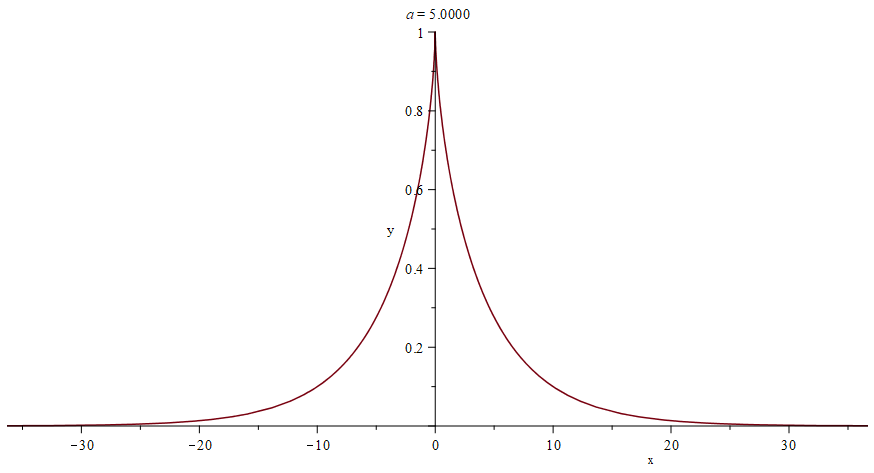
\includegraphics[width=1\linewidth]{../img/plot1.png}}
	\caption*{Рисунок 1 -- График трактрисы при $a=5$.}
	\label{ris:plot1}
\end{figure}


Если линия задана параметрически, то ее эволюта имеет уравнение:
\begin{align}
	X(t)=x(t)-y^{\prime} \frac{x^{2}+y^{\prime 2}}{x^{\prime} y^{\prime \prime}-x^{\prime \prime} y^{\prime}},\label{eq43}\\
	Y(t)=y(t)+x^{\prime} \frac{x^{2}+y^{2}}{x^{\prime} y^{\prime \prime}-x^{\prime \prime} y^{\prime}}.\label{eq44}
\end{align}

Подставляя уравнение трактрисы в (\ref{eq43}) и (\ref{eq44}) и сокращая, получим:
\begin{align}
	X(t)&=\frac{-\cos (t)^{3} a^{2}+\ln \left(\frac{1-\cos (t)}{\sin (t)}\right) a^{2}+\cos (t)^{3}+\cos (t) a^{2}-\cos (t)}{a},\label{eq45}\\
	Y(t)&={\frac {1+ \left( {a}^{2}-1 \right)  \left( \cos \left( t \right) 
			\right) ^{4}}{\sin \left( t \right) }}.\label{eq46}	
\end{align}


Избавляясь в полученной системе от $t$ придём к уравнению эволюты, зависящей только от $x$:
\begin{equation}\label{eq47}
	evoluta(x) = a\cdot \cosh{\frac{x}{a}}.
\end{equation}

\begin{figure}[h]
	\center{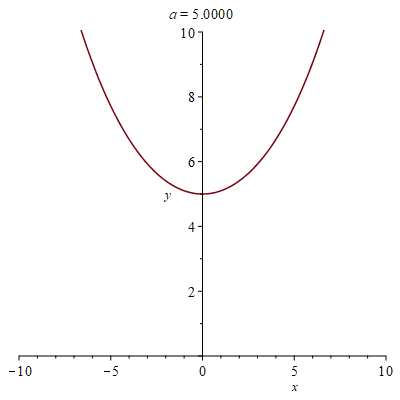
\includegraphics[width=0.85\linewidth]{../img/plot2.png}}
	\caption*{Рисунок 2 -- График эволюты трактрисы при $a=5$.}
	\label{ris:plot2}
\end{figure}


Получили, что эволютой трактрисы является цепная линия.

Определение 15. Цепная линия — линия, форму которой принимает гибкая однородная нерастяжимая тяжёлая нить или цепь (отсюда название) с закреплёнными концами в однородном гравитационном поле. Является плоской кривой. Её уравнением является (\ref{eq47}).



Вращая полученную эволюту вокруг оси $OX$ получаем поверхность вращения, называемую катеноидом. Катеноид можно задать параметрически:
\begin{align}
	x_{kat}(u,v) &= a\cdot \cosh{\frac{v}{a}}\cos{u},\label{eq48}\\
	y_{kat}(u,v) &= a\cdot \cosh{\frac{v}{a}}\sin{u},\label{eq49}\\
	z_{kat}(u,v) &= u,\label{eq50}
\end{align}
где $-\pi \leq u \leq \pi$ и $v \in \mathbb{R}$.


Построим полученную поверхность.
\begin{figure}[h]
	\center{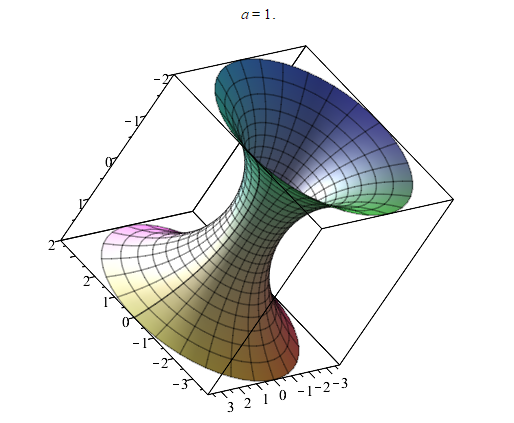
\includegraphics[width=0.85\linewidth]{../img/plot3.png}}
	\caption*{Рисунок 3 -- Катеноид при $a=1$.}
	\label{ris:plot3}
\end{figure}


Для вычисления Гауссовой и средней кривизн воспользуемся формулами из (\cite{Oprea}), позволяющими написать универсальный программный код.


Пусть $K$ -- Гауссова кривизна, а $H$ -- средняя. Введём дополнительные обозначения:

\begin{align}
	E &= x_u \cdot x_u, \label{eq51}\\
	F &= x_u \cdot x_v, \label{eq52}\\
	G &= x_v \cdot x_v, \label{eq53}\\
	l &= U \cdot x_{uu}, \label{eq54}\\
	m &= U \cdot x_{uv}, \label{eq55}\\
	n &= U \cdot x_{vv}, \label{eq56}
\end{align}
где $U$ -- единичный вектор нормали к поверхности:
\begin{equation}
	U = \frac{x_u \times x_v}{|x_u \times x_v|}.\label{eq 57}
\end{equation}


Тогда Гауссова кривизна будет рассчитываться как
\begin{equation}\label{eq58}
	K = \frac{lm - m^2}{EG-F^2},
\end{equation}
а средняя кривизна:
\begin{equation}\label{eq59}
	H = \frac{Gl + En -2Fm}{2(EG-F^2)}.
\end{equation}

Рассчитаем введённые выше величины для нашего катеноида (\ref{eq48})-(\ref{eq50}):

\begin{equation}\label{eq60}
\begin{split}
	E &= x_u \cdot x_u = \\
	&= (1, \sinh{\frac{u}{a}} \cos{v}, \sinh{\frac{u}{a}} \sin{v}) \cdot (1, \sinh{\frac{u}{a}} \cos{v}, \sinh{\frac{u}{a}} \sin{v})  = \\
	&= 1+\sinh{\frac{u}{a}}^2\cdot\cos^2{v}+\sinh{\frac{u}{a}}^2\cdot\sin^2{v}. \\
\end{split}
\end{equation}

\begin{equation}\label{eq61}
\begin{split}
	F &= x_u \cdot x_v = \\
	&= (1, \sinh{\frac{u}{a}} \cos{v}, \sinh{\frac{u}{a}} \sin{v}) \cdot (0, -a\cosh{\frac{u}{a}} \sin{v}, a\cosh{\frac{u}{a}} \cos{v})=\\
	&= 0. 
\end{split}
\end{equation}

\begin{equation}\label{eq62}
\begin{split}
	G &= x_v \cdot x_v = \\
	&= (0, -a\cosh{\frac{u}{a}} \sin{v}, a\cosh{\frac{u}{a}} \cos{v}) \cdot (0, -a\cosh{\frac{u}{a}} \sin{v}, a\cosh{\frac{u}{a}} \cos{v})  = \\	&= a^2 \cosh^2{\frac{u}{a}} \sin^2{v} + a^2 \cosh^2{\frac{u}{a}} \cos^2{v}.\\
\end{split}
\end{equation}


\begin{equation}\label{eq63}
\begin{split}
	U &= \frac{x_u \times x_v}{|x_u \times x_v|} = \\
	&= \frac{(0, -a\cosh{\frac{u}{a}} \sin{v}, a\cosh{\frac{u}{a}} \cos{v}) \times (0, -a\cosh{\frac{u}{a}} \sin{v}, a\cosh{\frac{u}{a}} \cos{v}) }{|(0, -a\cosh{\frac{u}{a}} \sin{v}, a\cosh{\frac{u}{a}} \cos{v}) \times (0, -a\cosh{\frac{u}{a}} \sin{v}, a\cosh{\frac{u}{a}} \cos{v})|} = \\
	&= \frac{(a\cosh{\frac{u}{a}}\sinh{\frac{u}{a}}, -a \cosh{\frac{u}{a}}\cos{v}, -a \cosh{\frac{u}{a}} \sin{v})}{\sqrt{\cosh^4{\frac{u}{a}}a^2}} = \\
	&= (\frac{\sinh{\frac{u}{a}}}{\cosh{\frac{u}{a}}},-\frac{\cos{v}}{\cosh{\frac{u}{a}}} ,-\frac{\sin{v}}{\cosh{\frac{u}{a}}}).
\end{split}
\end{equation}

\begin{equation}\label{eq64}
\begin{split}
	l &= U \cdot x_{uu} = \\
	&=  (\frac{\sinh{\frac{u}{a}}}{\cosh{\frac{u}{a}}},-\frac{\cos{v}}{\cosh{\frac{u}{a}}} ,-\frac{\sin{v}}{\cosh{\frac{u}{a}}}) \cdot (0, \frac{\cosh{\frac{u}{a}}\cos{v}}{a}, \frac{\cosh{\frac{u}{a}}\sin{v}}{a}) = \\
	&= -\frac{1}{a}.
\end{split}
\end{equation}

\begin{equation}\label{eq65}
\begin{split}
	m &= U \cdot x_{uv} = \\
	&=  (\frac{\sinh{\frac{u}{a}}}{\cosh{\frac{u}{a}}},-\frac{\cos{v}}{\cosh{\frac{u}{a}}} ,-\frac{\sin{v}}{\cosh{\frac{u}{a}}}) \cdot (0, -\sinh{\frac{u}{a}}\sin{v}, \sinh{\frac{u}{a}}\cos{v}) = \\
	&= 0.
\end{split}
\end{equation}


\begin{equation}\label{eq66}
\begin{split}
	n &= U \cdot x_{vv} = \\
	&=  (\frac{\sinh{\frac{u}{a}}}{\cosh{\frac{u}{a}}},-\frac{\cos{v}}{\cosh{\frac{u}{a}}} ,-\frac{\sin{v}}{\cosh{\frac{u}{a}}}) \cdot (0, -a\cosh{\frac{u}{a}}\cos{v}, -a\cosh{\frac{u}{a}}\sin{v}) = \\
	&= a.
\end{split}
\end{equation}

Теперь мы можем рассчитать Гауссову кривизну по формуле (\ref{eq58}):
\begin{equation}\label{eq67}
	K = \frac{lm - m^2}{EG-F^2} = - \frac{1}{\cosh^4{\frac{u}{a}}a^2}.
\end{equation}

И среднюю кривизну по формуле (\ref{eq59}):
\begin{equation}\label{eq68}
	H = \frac{Gl + En -2Fm}{2(EG-F^2)} = 0.
\end{equation}


Также из \cite{Oprea} известно, что скалярная кривизна равняется удвоенной гауссовой кривизне для римановых многообразий. Так что, обозначая скалярную кривизну за $SK$ имеем:
\begin{equation}\label{eq69}
	SK = 2K  = - \frac{2}{\cosh^4{\frac{u}{a}}a^2}.
\end{equation}




\clearpage
\addcontentsline{toc}{section}{Список использованных источников}
\begin{thebibliography}{3}
\bibitem{Dimitrienko}
	Димитриенко Ю.И. Тензорное исчисление: Учеб.пособие для вузов. М.: Высш,	шк., 2001, 575 с.
\bibitem{Petrov}
	Петров А.З. Пространства Эйнштейна. М.: Физматгиз, 1961, 464 с.
\bibitem{Rashevskiy}
	Рашевский П.К. Риманова геометрия и тензорный анализ. М.: Наука, 1967, 664 с.
\bibitem{Shipov}
	Шипов Г.И. Теория физического вакуума. НТ-Центр, 1993, 362 с.
\bibitem{Oprea}
	Шипов Г.И. Теория физического вакуума. НТ-Центр, 1993, 362 с.
\end{thebibliography}

\end{document}